\documentclass[a4paper]{article}

%% Language and font encodings
\usepackage[english]{babel}
\usepackage[utf8x]{inputenc}
\usepackage[T1]{fontenc}

%% Sets page size and margins
\usepackage[a4paper,top=3cm,bottom=2cm,left=3cm,right=3cm,marginparwidth=1.75cm]{geometry}

%% Useful packages
\usepackage{amsmath}
\usepackage{graphicx}
\usepackage[colorinlistoftodos]{todonotes}
\usepackage[colorlinks=true, allcolors=blue]{hyperref}

\title{Rapport TER\\ Plate-forme de calcul distribué en JavaScript}
%\title{Plate-forme de calcul javascript}
\author{Taoukilite Ahmed El Mahdi}

\begin{document}
\maketitle

\section{Présentation du projet}
\subsection{Contexte}
Le projet consiste à concevoir une plateforme de calcul distribuée, basé sur le volontariat, et qui permettrait au chercheurs d'avoir la puissance calculs de nombreux ordinateur personnels dans le monde entier. Cela est fait grâce a l'exploitation des navigateurs internet des volontaires qui joueront le rôle des workers en exécutant du code javascript qui recoivent de la plateforme. Les calculs seront effectué sur les machines volontaires et les résultats seront renvoyés à la plate-forme.

\subsection{Objectifs}

L'objectif de ce projet est de développer en premier temps un interface web qui permettra dans lancer un calcul avec un nombre de jobs, à partir d'un code javascript saisie par le chercheur (Figure \ref{fig:IntChercheur}). En effet un chercheur accéderas a l'interface web  puis saisiras le code des jobs donc le code qui seras exécuter sur chaque volontaire qui participe au calcul, la plate-forme créer le nombre de job choisie par le chercheur en envoyent des messages contenant le code javascript et l'id du job (Correlation id) aux serveur de file de messages.

La plateforme contiendras une deuxiéme interface web qui est l'interface volontaire (Worker), cet interface joueras le role de l'executeur en effet le volontaire se rendre sur le site de la plateforme, puis ainsi commenceras a participer au calcul en consommant les jobs créer par le chercheur. Ces jobs sont extrait du serveur de la file de message par le coté serveur de la plateforme ensuite ces jobs sont envoyer au volontaires (Workers) qui décortiqueront le message en retrouvant le code et l'id du job, puis le code javascript extrait seras evalué puis executer en fonction des paramétres en entrées (l'id du job) ou pas.

Un volontaire participe au calcul dés qu'il se connecte sur le interface volontaire de la plateforme, et se déconnecte quand il ferme l'interface.



\section{Fonctionnement}
\subsection{Acteurs}
La plate-forme (Figure 2 \ref{fig:ArchGenarale}) contient 4 types d'acteurs:
\begin{itemize}
\item Un acteur de type serveur web (type NodeJS) pour gérer les chercheurs et les volontaires, qui effectue les opérations suivantes:
\begin{itemize}

\item Interactions avec l'interface chercheur :
\begin{itemize}
\item Récupération du code JavaScript du calcul + le nombre de jobs a créer.
\item Creation et géneration des jobs d'un calcul.
\item Dépot de ces jobs dans la file de messages dédié au jobs.
\item Récupération des résultats des jobs a partir la file des résultats (un calcul se termine dés que les réponses de tout les jobs est reçu).
\end{itemize}

\item Interactions avec l'interface volontaire :
\begin{itemize}
\item Récupération des jobs à partir de la file des jobs.
\item Envoie des jobs aux volontaires.
\item Récupération des résultats du job exécuter par le volontaire.
\item Dépôts des résultats dans la file des résultats
\end{itemize} 

\item Un serveur web (type NodeJS) pour gérer les chercheurs, qui effectue les opérations suivantes:
\begin{itemize}
\item 
\item Génération et dépôt des jobs à la file des jobs.
\item Récupération des résultats du calcul a partir la file des résultats.
\end{itemize} 

\end{itemize}
  
\end{itemize} 
\subsection{Architecture de la plate-forme}




\subsection{Annexe}
\begin{figure}
\centering
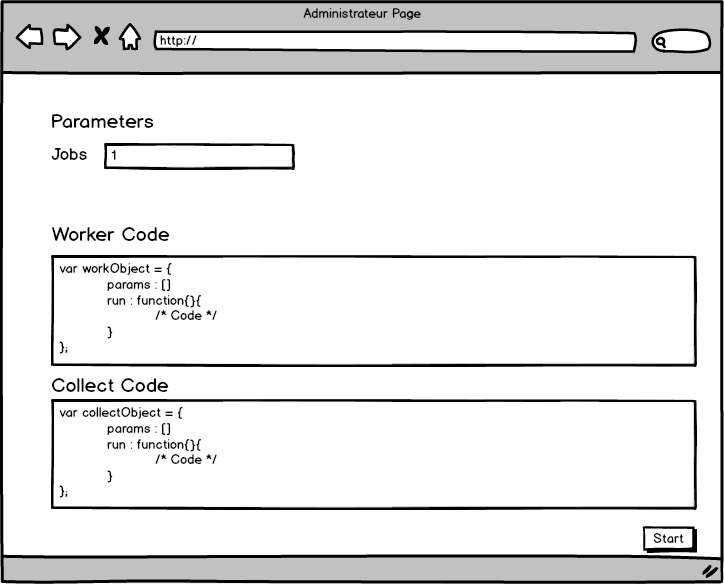
\includegraphics[width=0.6\textwidth]{IntChercheur.png}
\caption{\label{fig:IntChercheur}Prototype d'interface chercheur}
\end{figure}

\begin{figure}
\centering
\includegraphics[width=0.6\textwidth]{ArchGen.png}
\caption{\label{fig:ArchGenarale}Architecture générale de la plate-forme}
\end{figure}




\end{document}
